\RequirePackage{fix-cm}
\documentclass[11pt]{article}       % onecolumn (second format)
%\smartqed  % flush right qed marks, e.g. at end of proof
\usepackage{graphicx,multicol,lipsum,caption,authblk}
\usepackage{amsmath,booktabs,verbatim,tikz}
\usetikzlibrary{shapes.geometric, arrows,positioning,matrix,calc}
\usepackage{mathptmx}
\begin{document}
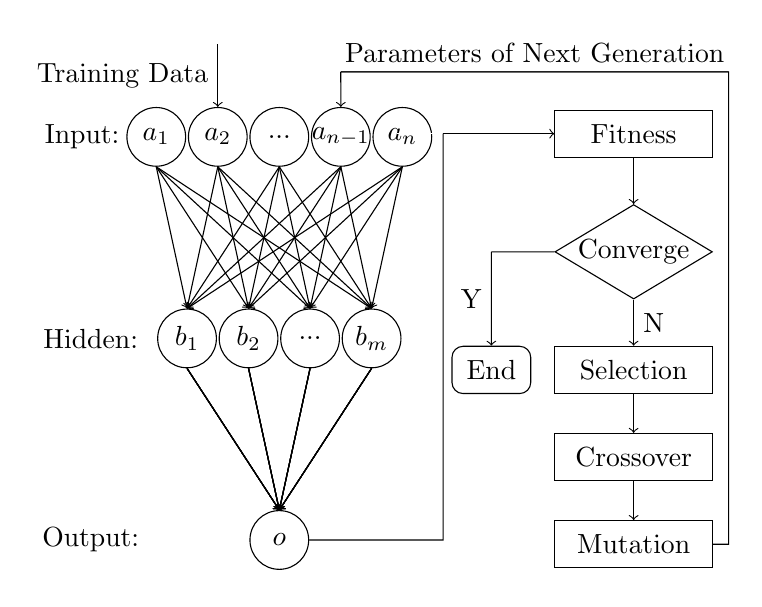
\begin{tikzpicture}
[
plain/.style={
  draw=none,
  fill=none,
  },
  remember picture,
net/.style={
  matrix of nodes,
  nodes={
    draw,
    circle,
    inner sep=7.5pt
    },
  nodes in empty cells,
  column sep=-10.5pt,
  row sep=1.8cm
  }
]
%\draw[help lines] (-3cm,-6cm) grid (6cm,3cm);
\matrix[net] (mat)
{
              & |[plain]| &           & |[plain]|  &           & |[plain]| &           &  |[plain]|      &               \\
    |[plain]| &           & |[plain]| &            & |[plain]| &           & |[plain]| &                 & |[plain]|     \\ 
    |[plain]| & |[plain]| & |[plain]| & |[plain]|  &           & |[plain]| & |[plain]| &  |[plain]|      & |[plain]|     \\ 
  };

  \node at ($(mat-1-1.west)+(-16pt,0)$) {Input: };
  \node at ($(mat-2-2.west)+(-24pt,0)$) {Hidden:};
  \node at ($(mat-3-2.west)+(-24pt,0)$) {Output:};
  \node at (mat-1-1.base) {$a_1$};
  \node at (mat-1-3.base) {$a_2$};
  \node at (mat-1-5.base) {...};
  \node at (mat-1-7.base) {$a_{n-1}$};
  \node at (mat-1-9.base) {$a_{n}$};
  \node at (mat-2-2.base) {$b_1$};
  \node at (mat-2-4.base) {$b_2$};
  \node at (mat-2-6.base) {$...$};
  \node at (mat-2-8.base) {$b_{m}$};
  \node at (mat-3-5.base) {$o$};

 \foreach \a in {1,3,5,7,9}{
    \foreach \b in {2,4,6,8}{
        \draw[->] (mat-1-\a.south) -- (mat-2-\b.north);
     }
 \foreach \c in {2,4,6,8}
 \draw[->] (mat-2-\c.south) -- (mat-3-5.north);
  }
  
  % write text
  \draw[<-] (mat-1-3.north) -- +(0,0.8cm) node[pos=0.5,auto=left] {Training Data} ;
  \coordinate (shift) at (4.5,2.6);
  \begin{scope}[shift=(shift)]
    \tikzstyle{startstop} = [rectangle, rounded corners, minimum width=1.0cm,minimum height=0.6cm, text centered, draw=black]
    \tikzstyle{io} = [trapezium, trapezium left angle=70, trapezium right angle=110, minimum width=2cm, minimum height=0.6cm, text centered, draw=black]
    \tikzstyle{process} = [rectangle, minimum width=2cm, minimum height=0.6cm, text centered, draw=black]
    \tikzstyle{decision} = [diamond,minimum width=2cm, minimum height=1.2cm, draw=black]
    \node (fitness) [process] {Fitness};
    \node[yshift=-0.5cm] (decision) [decision, below of=fitness] {} node at (decision.base) {Converge};
    \node[yshift=-0.5cm] (selection) [process, below of=decision] {Selection};
    \node (crossover) [process] at ($(selection.south)+(0,-0.8cm)$) {Crossover};
    \node (mutation) [process] at ($(crossover.south)+(0,-0.8cm)$)  {Mutation};
    \node (end) [startstop] at ($(selection.west)+(-0.8cm,0cm)$) {End};

    \draw [->] (fitness) -- (decision);
    \draw [->] (decision.south) -- (selection.north) node[auto=left,pos=0.5]{N};
    \draw [->] (selection.south) -- (crossover.north);
    \draw [->] (crossover.south) -- (mutation.north);

    % draw intersection
    \draw [white] (decision.west) -- ++(-1.5cm,0) coordinate (A);
    \draw [white] (end.north) -- ++(0,3cm) coordinate (B);
    \draw[<-] (end.north) -- (intersection cs: first line={(decision.west)--(A)}, second line={(end.north)--(B)}) node[pos=0.5,auto=left] {Y} coordinate (C);
    \draw (decision.west) -- (C);
    % draw intersection
    \draw[white] (mat-3-5.east) -- ++(1.7cm,0) coordinate (D) -- ++(0,6cm) coordinate (E);
    \draw[white] (fitness.west) -- ++(-2cm,0) coordinate (F);
    \draw (mat-3-5.east) -- ++(1.7cm,0) -- (intersection cs: first line={(fitness.west)--(F)}, second line={(D)--(E)});
    \draw[<-] (fitness.west) -- (intersection cs: first line={(fitness.west)--(F)}, second line={(D)--(E)});
    % draw intersection
    \draw[white] (mutation.east) -- ++(0.2cm,0) -- ++(0,6cm) coordinate (G) -- ++(-6cm,0) coordinate (H);
    \draw[white] (mat-1-7.north) coordinate (I) -- ++(0,1cm) coordinate (J);
    \draw (mutation.east) -- ++(0.2cm,0) -- ++(0,6cm) -- (intersection cs: first line={(G)--(H)}, second line={(I)-- (J)}) coordinate (L);
    \draw (G) -- (L) node[pos=0.5,auto=right] {Parameters of Next Generation};
    \draw[<-] (mat-1-7.north) -- (L);
  \end{scope}
\end{tikzpicture}
\end{document}

